% EHB326E HW2 — based on the official GSTL-ITU/uBee Homework_N/report/latex_src/main_en.tex
% Template source: https://github.com/GSTL-ITU/uBee/blob/main/Homework_N/report/latex_src/main_en.tex
% Report scope: simulations and synthesis only; no physical FPGA validation.
\documentclass[12pt,a4paper]{article}
\usepackage[T1]{fontenc}
\usepackage[utf8]{inputenc}
\usepackage[english]{babel}
\usepackage{mathptmx}
\usepackage[a4paper,margin=2.5cm,headheight=16pt]{geometry}
\usepackage{graphicx,caption,booktabs,tabularx,enumitem}
\usepackage{needspace}
\usepackage{tikz}
\usetikzlibrary{arrows.meta,positioning,shapes.geometric}
\usepackage{xcolor}
\definecolor{baslik}{HTML}{17365D}
\usepackage{titlesec}
\titleformat{\section}{\Large\bfseries\color{baslik}}{\thesection}{.7em}{}
\titleformat{\subsection}{\large\bfseries\color{baslik}}{\thesubsection}{.7em}{}
\usepackage{fancyhdr,lastpage}
\pagestyle{fancy}
\fancyhf{}
\newcommand{\ogrenciad}{Arda Y\"uce}
\newcommand{\ogrencino}{040230045}
\fancyhead[L]{\small \ogrenciad\enspace--\enspace\ogrencino}
\fancyhead[R]{\small EHB326E}
\fancyfoot[C]{\thepage\ / \pageref{LastPage}}
\renewcommand{\headrulewidth}{0.4pt}
\usepackage{ragged2e}
\AtBeginDocument{\justifying}
\usepackage{hyperref}
\hypersetup{colorlinks=true,linkcolor=baslik,urlcolor=baslik,citecolor=baslik}
\newcommand{\raporbasligi}{Dijkstra Algorithm and microBee Profile Selection}
% Conservative layout adjustments: keep original class, margins, font and section styles.
\captionsetup{font=small,labelfont=bf,skip=4pt}
\setlength{\textfloatsep}{9pt plus 2pt minus 2pt}
\setlength{\floatsep}{8pt plus 2pt minus 2pt}
\setlength{\intextsep}{8pt plus 2pt minus 2pt}
\setlength{\parskip}{0pt}
\setlist{nosep,leftmargin=*}
\renewcommand{\arraystretch}{1.08}

\begin{document}
\begin{center}
{\Large\bfseries Istanbul Technical University}\\[5pt]
{\large EHB326E -- Assignment 2 Report}\\[13pt]
{\LARGE\bfseries\color{baslik}\raporbasligi}\\[11pt]
\ogrenciad\quad(\ogrencino)\\[5pt]
3 November 2026
\end{center}
\vspace{0.5em}

\section{Abstract}
This study implements Dijkstra's single-source shortest-path algorithm in RV32IMC assembly on the configurable microBee processor and compares execution performance against FPGA resource cost. A seven-node functional test and a deterministic 32-node graph were verified in Vivado XSim against independent reference algorithms. CPU cycle/retirement counters and branch events provided execution measurements, while Vivado synthesis reported resource utilization for the Arty A7-100 target. Five configurations passed verification and synthesis; a planned gshare configuration was excluded after an XSim elaboration incompatibility was traced to protected core RTL. A weighted-sum multi-criteria evaluation selected the reduced-DMEM profile (P6) for the tested workload: it retained the reference execution time while lowering BRAM use by 25\%. This selection is conditional on the application's reduced 32\,KiB data-memory footprint.

\section{Objective and Requirements}
The task is to execute Dijkstra's algorithm correctly on microBee and choose a processor configuration that balances computation cost with limited FPGA resources. Dijkstra's algorithm finds minimum-cost routes from a source in a non-negative weighted graph \cite{dijkstra1959}. For a fixed workload, the study aims to (i) implement and verify the algorithm in assembly, (ii) compare the effect of configurable branch prediction and data-memory size, and (iii) select a suitable profile by an explicit multi-criteria decision procedure. All candidate designs retain the provided processor ISA, pipeline and core RTL, in accordance with course rules \cite{course}. Identical software, benchmark inputs, measurement boundaries and FPGA target are used for quantitative comparison.

\section{Method and System Design}
\subsection{Algorithm and SoC organization}
A square adjacency matrix represents the graph; a linear scan chooses the unvisited node with minimum tentative distance, followed by relaxation of its outgoing edges. The algorithm maintains \texttt{dist}, \texttt{visited} and \texttt{parent} arrays. Its time complexity is $O(N^2)$ with $O(N^2)$ matrix storage. This variant was chosen instead of a priority queue because its addressing, control flow and memory layout are simple to implement and inspect in assembly. Absent edges use \texttt{0xFFFFFFFF}; unreachable distances use \texttt{0x7FFFFFFF}. The implementation also guards against distance overflow.

The processor executes instructions from IMEM at \texttt{0x80000000} and reads the graph from DMEM at \texttt{0x20000000}. Completion and status words, plus the result arrays, are checked by an external testbench. Figure~\ref{fig:soc} summarizes the actual SoC organization, including the AXI UART Lite, clock/reset path and read-only simulation observation. The 100\,MHz clock is the configured simulation/clocking target, \emph{not} a demonstrated post-route timing result. microBee architectural and configuration details follow the official project sources \cite{ubee}.

\begin{figure}[!htbp]\centering
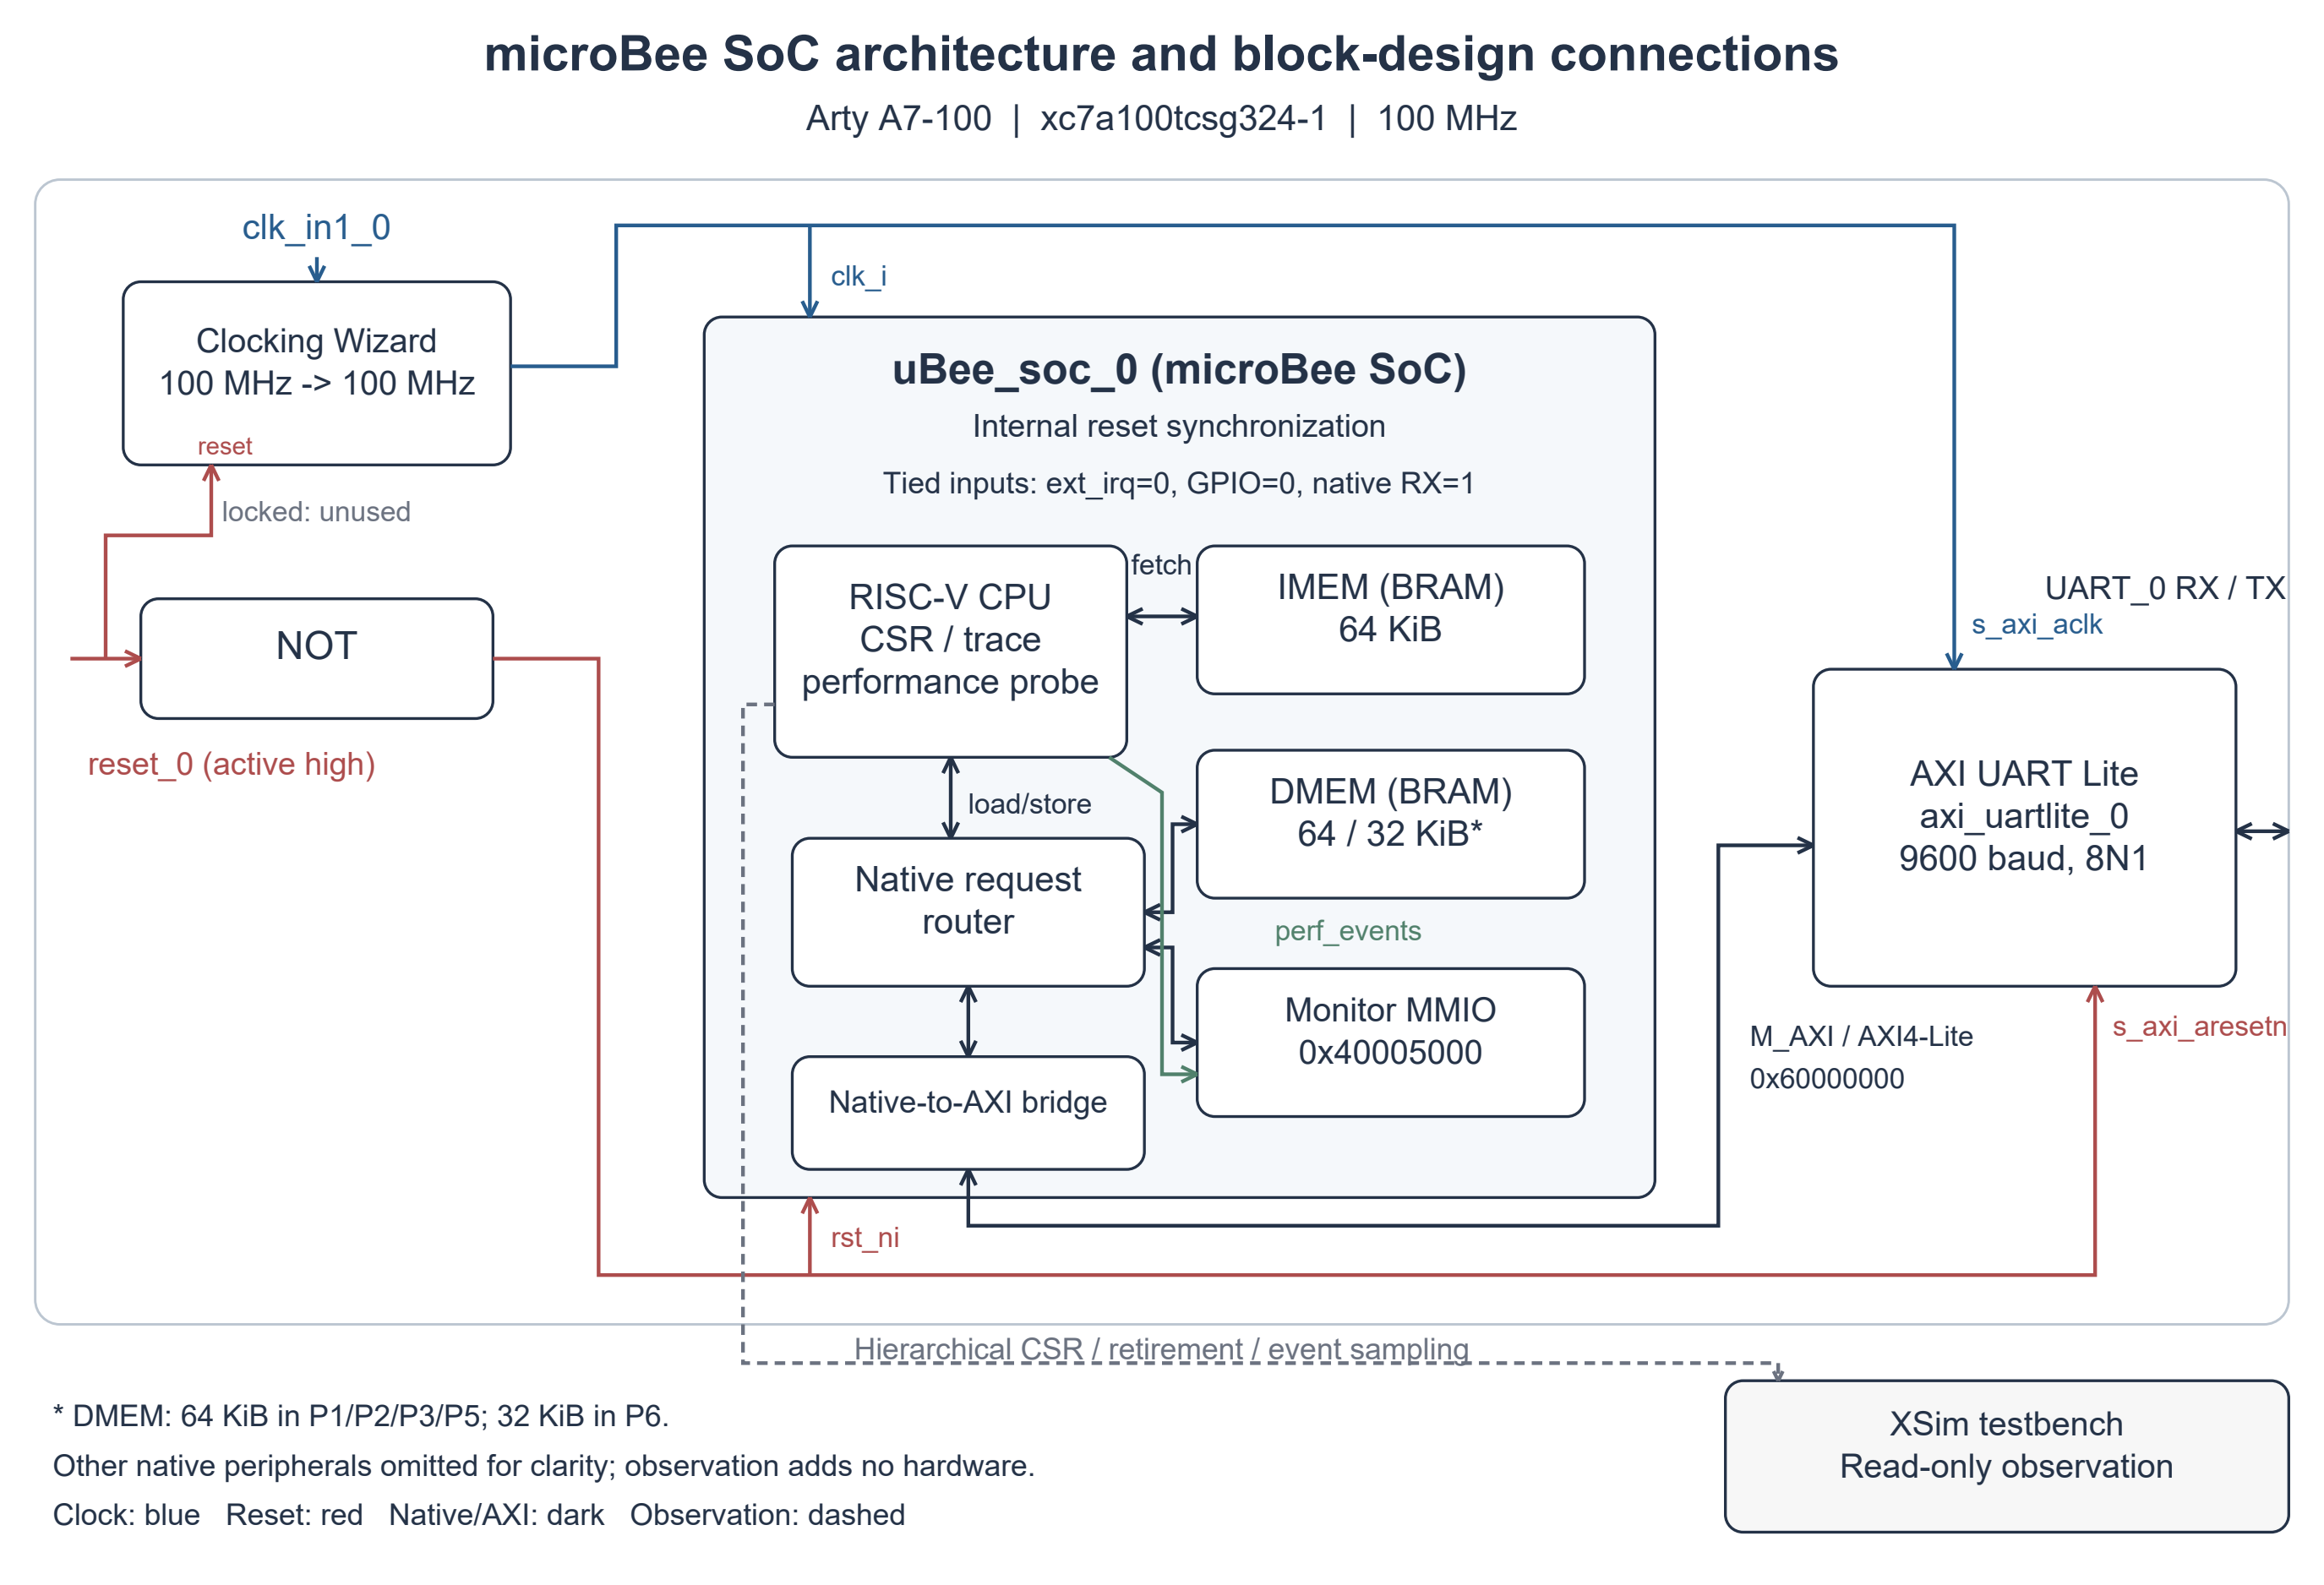
\includegraphics[width=\linewidth]{figure1_microbee_architecture.png}
\caption{microBee SoC, memory/peripheral paths and non-intrusive RTL observation. The diagram summarizes the tested block design, not physical-board validation.}
\label{fig:soc}
\end{figure}

\subsection{Implementation and configuration choices}
A single RV32IMC-compatible assembly image reads graph size, source and matrix, initializes the working arrays, then repeatedly selects and relaxes vertices. The completed distances and predecessors are stored in DMEM, followed by \texttt{done/status} publication. The tested software was kept unchanged between processor profiles. Table~\ref{tab:profiles} specifies the controlled parameters. P1 is the baseline; P2/P3 alter predictor capacity, P4 was intended to evaluate gshare, P5 disables prediction, and P6 halves DMEM capacity. All profiles retain \texttt{IMEM\_WORDS=16384}, \texttt{MONITOR\_ENABLE=1}, \texttt{MUL\_ENABLE=1} and \texttt{DIV\_ENABLE=1}; other parameters remain at their defaults.

\begin{table}[!htbp]\centering\small
\caption{Planned processor profiles (P4 not quantitatively evaluated).}\label{tab:profiles}
\begin{tabular}{@{}lrrrrr@{}}\toprule
Profile & BP enable & Entries & Gshare & GHR width & DMEM words\\\midrule
P1 & 1 & 128 & 0 & 5 & 16384\\
P2 & 1 & 32 & 0 & 5 & 16384\\
P3 & 1 & 256 & 0 & 5 & 16384\\
P4 (planned) & 1 & 128 & 1 & 5 & 16384\\
P5 & 0 & 128 & 0 & 5 & 16384\\
P6 & 1 & 128 & 0 & 5 & 8192\\\bottomrule
\end{tabular}
\end{table}

\Needspace{12\baselineskip}
\section{Simulation and Findings}
\subsection{Benchmarks and functional behavior}
A seven-node graph initially tested path reconstruction and an unreachable vertex. From source 0, the expected distance vector was $[0,7,9,20,20,11,\infty]$; the shortest route to node 4 was $0\!\rightarrow\!2\!\rightarrow\!5\!\rightarrow\!4$ with cost 20. Both the initial run and the reset/reload run passed.

The common performance workload was a deterministic, undirected 32-node graph constructed as a $4\times8$ grid with selected diagonal edges (Figure~\ref{fig:graph}). Its 70 edges represent 14.11\% of all $32\cdot31/2=496$ possible undirected pairs. Edge weights are non-negative and nonuniform, source node 0 is fixed, and the graph/memory-image data are identical across profiles. This controls differences unrelated to the CPU configuration.

\begin{figure}[!htbp]\centering
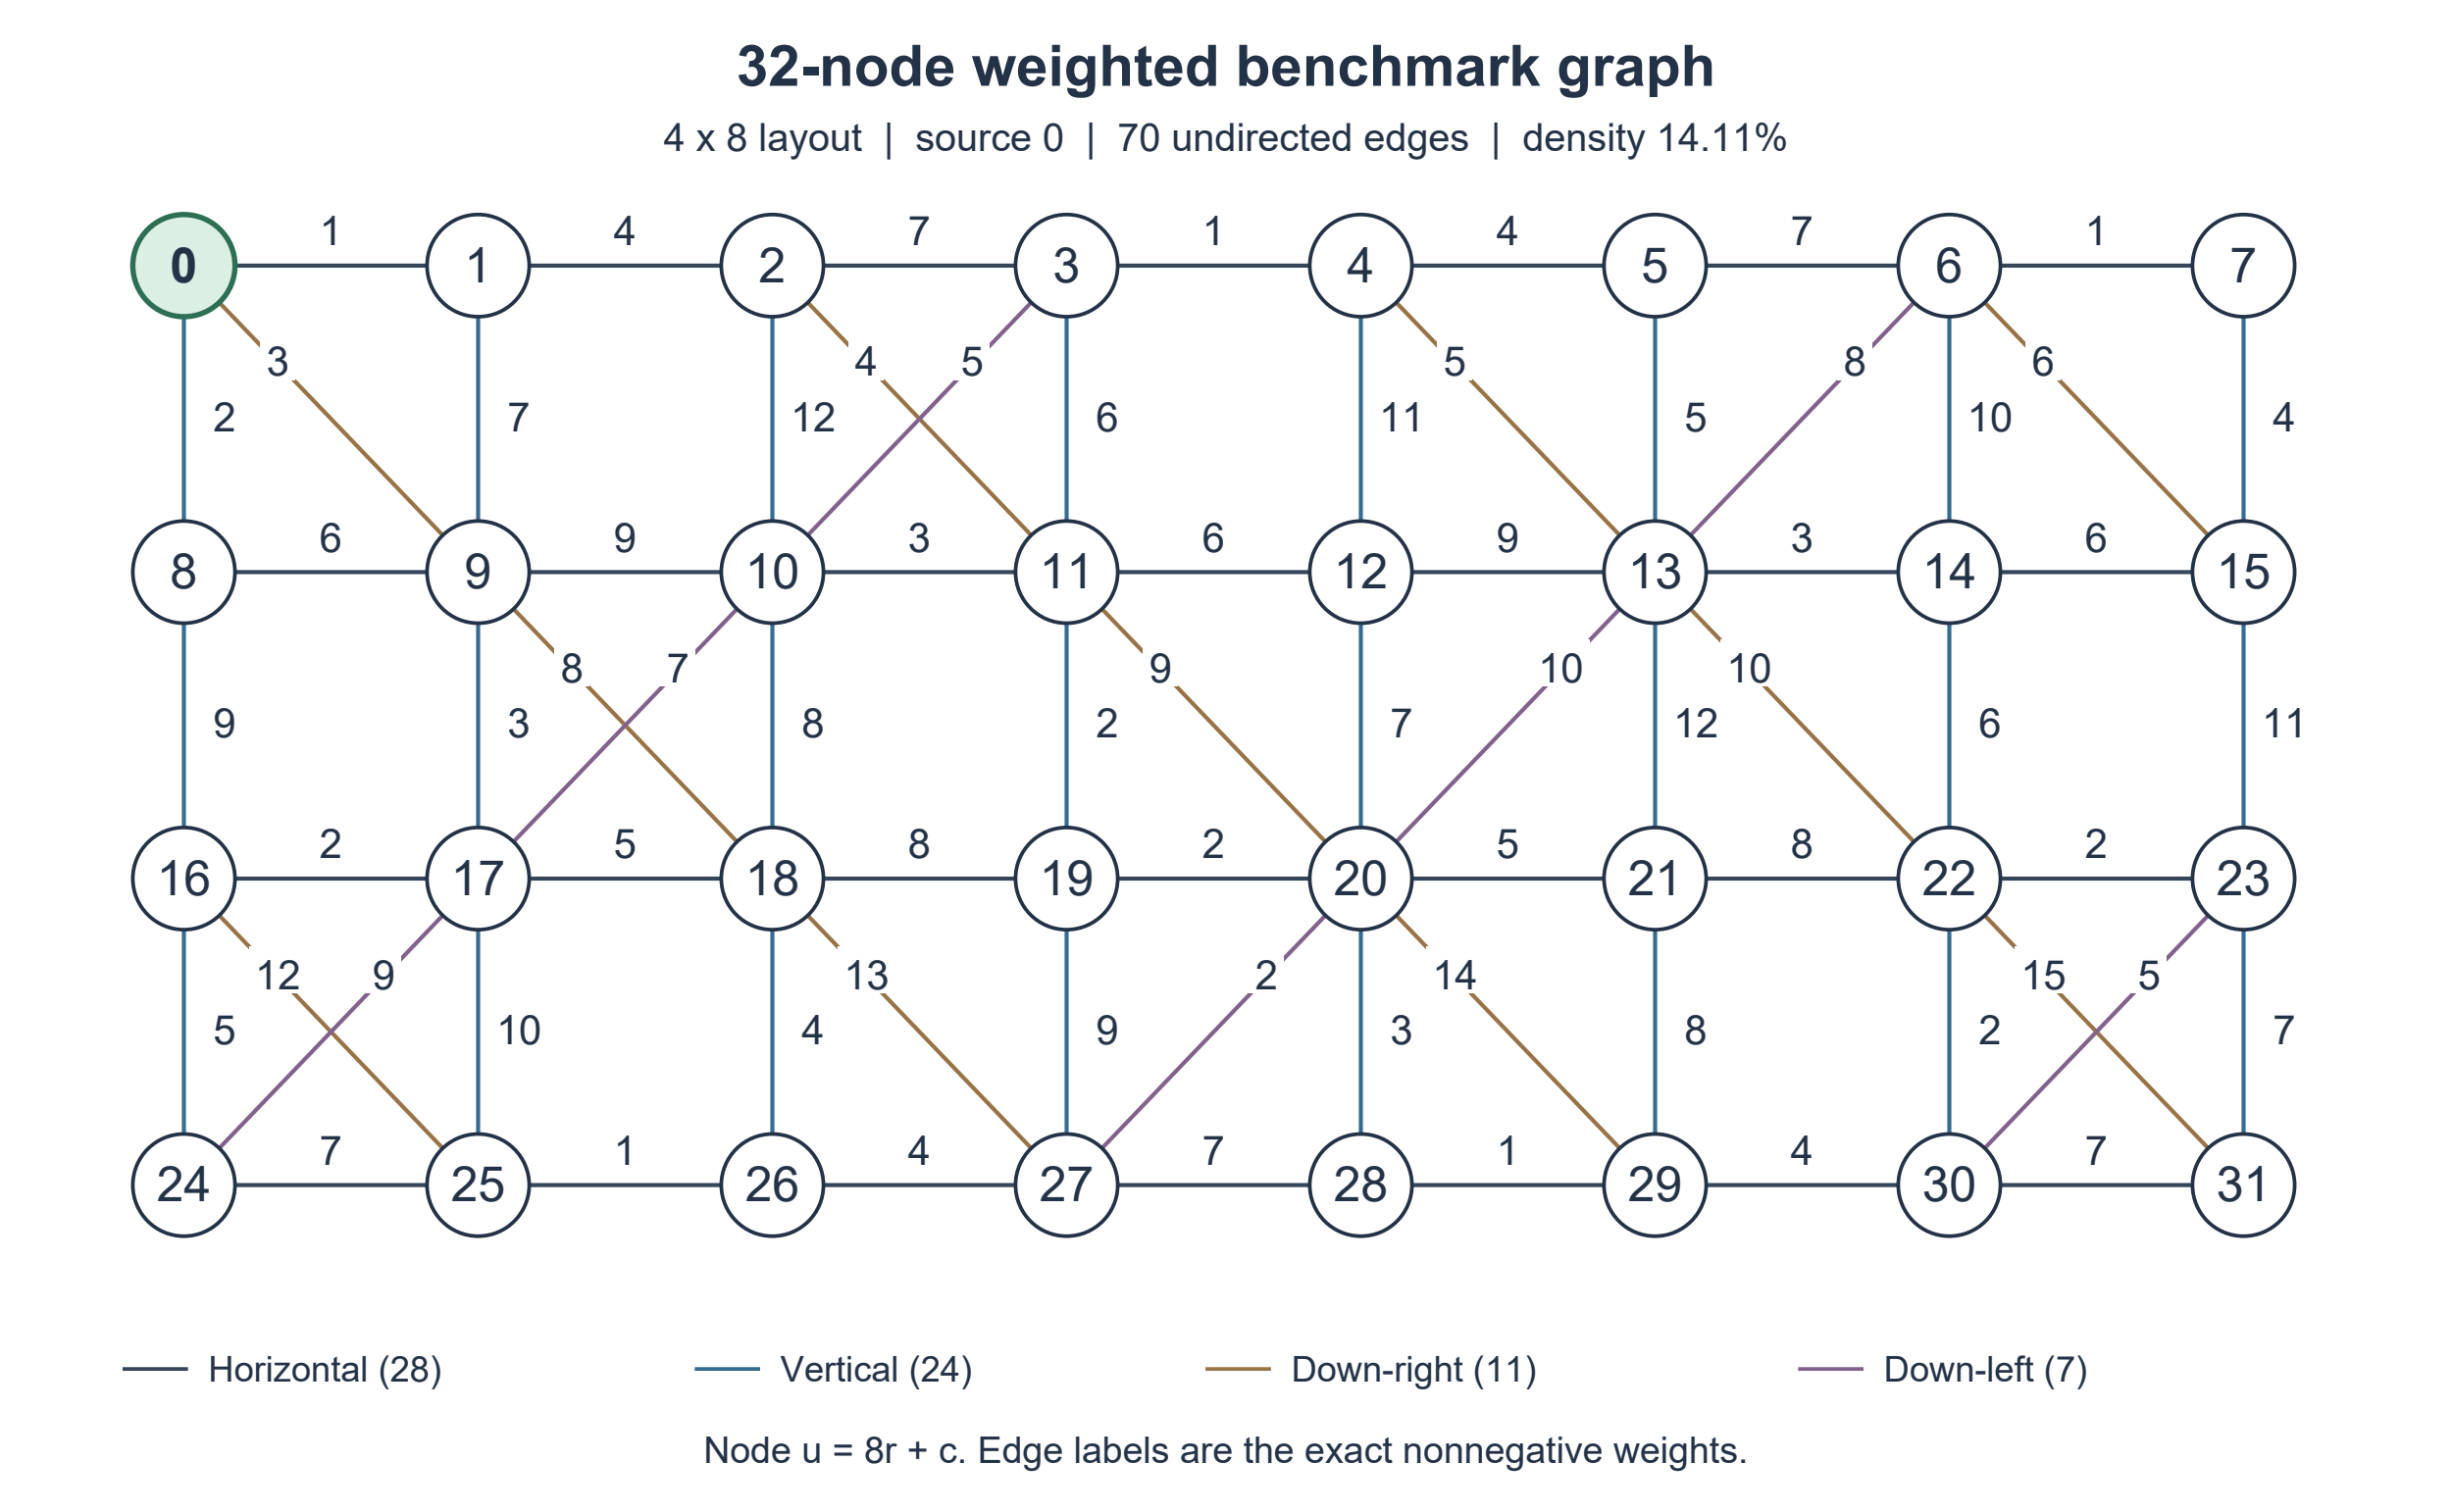
\includegraphics[width=\linewidth]{figure2_n32_weighted_graph.png}
\caption{Deterministic 32-node benchmark: actual topology and weights, with source node 0 highlighted.}
\label{fig:graph}
\end{figure}

\subsection{Performance measurement}
Vivado/XSim 2025.2 was used to observe the real RTL execution. The measurement interval extends from the accepted fetch of the first algorithm instruction to retirement of the final exit branch. It excludes reset, memory-image loading, result publication and the terminal idle loop. The 64-bit \texttt{mcycle} and \texttt{minstret} differences give window cycles and retired instructions; branch/taken/correct/misprediction events are collected from existing RTL signals without inserting measurement instructions into the assembly program. Cycle counts were cross-checked with clock edges and timestamps; retirements and branch events were checked against the execution trace. The testbench accessed the existing hardware CSR counter signals through hierarchical RTL references, including the mcycle and minstret debug outputs. Therefore, performance measurement was performed externally during simulation rather than through CSR-reading instructions embedded in the assembly program.

The 32-node interval includes 17,531 retired instructions, of which 17,528 belong to Dijkstra; three preceding preparation instructions retire inside the window because the pipeline overlaps the measurement boundary. Thus $\mathrm{CPI}_{\rm window}=\Delta mcycle/\Delta minstret$ is a \emph{window-based} value, not an isolated drained-kernel CPI. All five measured profiles retire 5,324 conditional branches (3,961 taken and 1,363 not taken). Table~\ref{tab:results} and Figure~\ref{fig:results} report the observed values and whole-SoC post-synthesis utilization.

\begin{table}[!htbp]\centering\footnotesize
\caption{32-node performance and Arty A7-100 synthesis results. BRAM is in RAMB36-equivalent tiles.}\label{tab:results}
\resizebox{\linewidth}{!}{%
\begin{tabular}{@{}lrrrrrrr@{}}\toprule
Profile & Cycles & CPI & Miss (\%) & LUT & FF & BRAM & DSP\\\midrule
P1 & 42,044 & 2.398 & 16.28 & 6,569 & 4,482 & 32 & 4\\
P2 & 42,139 & 2.404 & 16.89 & 6,299 & 4,284 & 32 & 4\\
P3 & 42,044 & 2.398 & 16.28 & 6,947 & 4,739 & 32 & 4\\
P5 & 48,528 & 2.768 & N/A & 6,019 & 4,023 & 32 & 4\\
P6 & 42,044 & 2.398 & 16.28 & 6,574 & 4,473 & 24 & 4\\\bottomrule
\end{tabular}}
\end{table}

\begin{figure}[!htbp]\centering
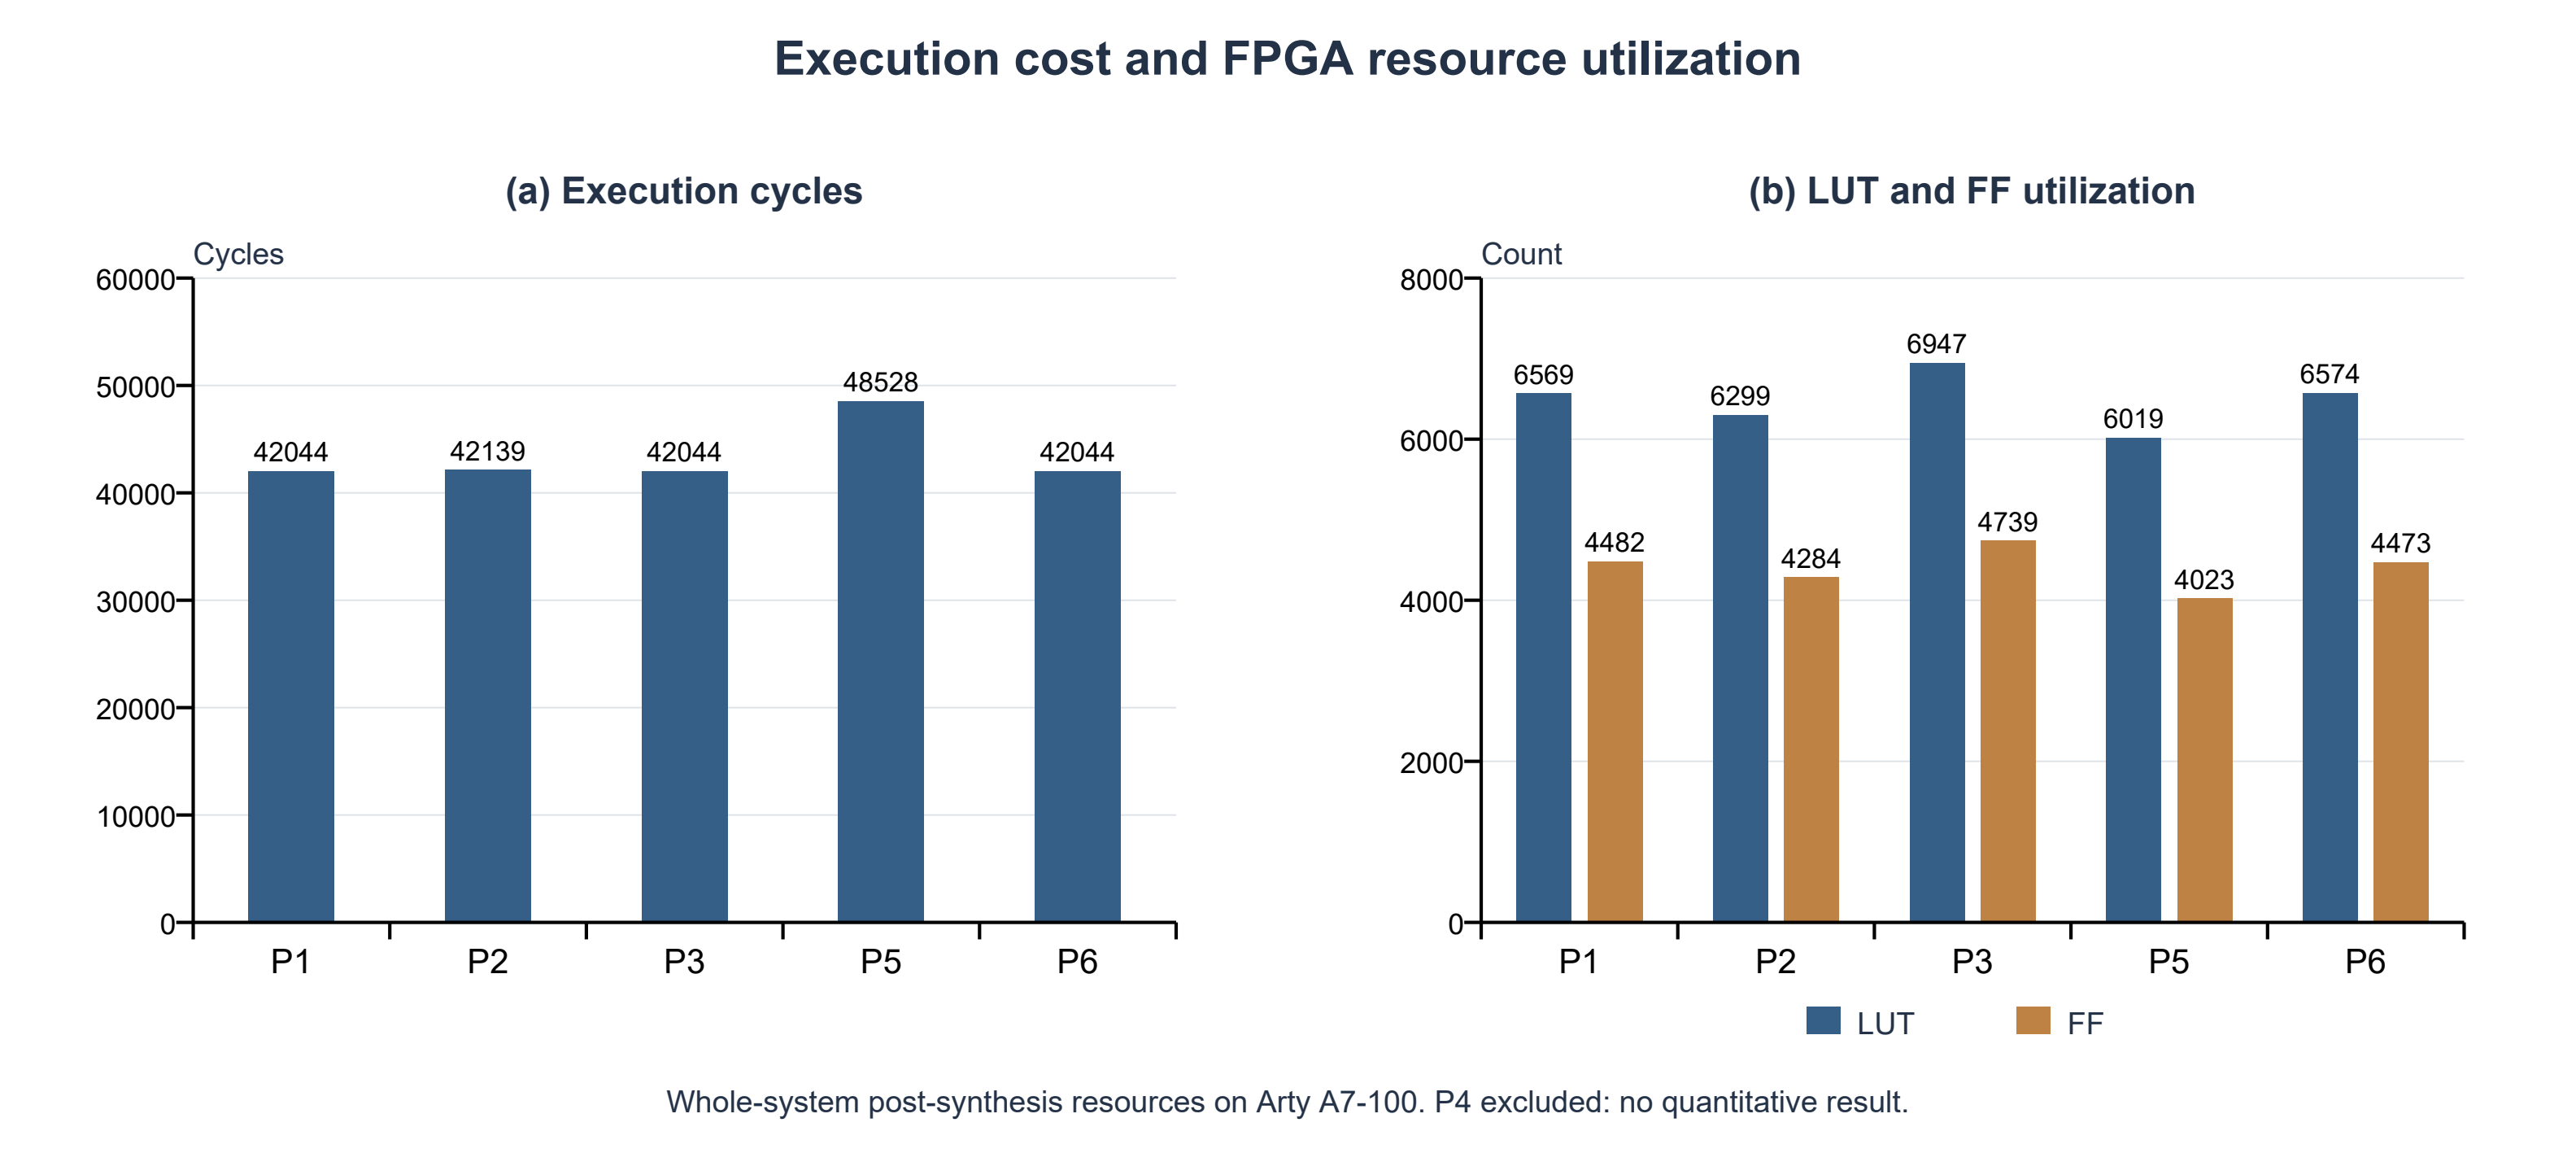
\includegraphics[width=\linewidth]{figure3_performance_resources.png}
\caption{Execution cycles and LUT/FF counts for the five successfully evaluated profiles.}
\label{fig:results}
\end{figure}

\section{Verification and Evaluation}
\subsection{Correctness, interpretation and limitations}
XSim results for P1, P2, P3, P5 and P6 passed distance, predecessor-chain, visitation, completion/status, trap and timeout checks. Independent Bellman--Ford and Floyd--Warshall calculations confirmed expected shortest paths; two reset/reload passes agreed for each verified profile. The testbench also checked instruction activity so that correct outputs could not be attributed merely to preloaded data.

P2 uses 4.1\% fewer LUTs than P1 but incurs 32 additional branch mispredictions (899 vs. 867) and 95 additional cycles (+0.23\%). Their ratio is approximately 2.97 cycles per additional misprediction, not an independently measured penalty. P3 provides no prediction or cycle benefit despite higher resource use. Disabling prediction (P5) increases execution time by 15.4\% while reducing logic resources; prediction accuracy is not applicable to P5. P6 retains P1's 42,044 cycles while reducing BRAM from 32 to 24 tiles with nearly unchanged LUT/FF usage. CPI also includes other execution stalls, which were not separately characterized.

P4 was intended to test gshare prediction. Its original RTL activated an XSim 2025.2 elaboration error because the simulator does not support directly slicing a concatenation expression. The failure was traced to the global-history update and a functionally equivalent assignment/truncation form was identified as a possible compatibility fix. However, applying it would require editing protected microBee core RTL; course rules forbid such modification \cite{course}. Consequently, P4 was not evaluated or assigned fabricated results. The proposed fix was \emph{not} used in the reported experiments.

P6 halves configured DMEM from 64 to 32\,KiB. The tested program makes no stack accesses and its actual data accesses fit within the smaller region, so the observed result is valid for this benchmark. Nevertheless, BRAM savings are a \emph{direct consequence of provisioning less memory}, not a stand-alone architectural efficiency improvement; the result cannot be generalized to programs requiring more than 32\,KiB. Utilization figures are post-synthesis whole-SoC results, not timing-closed implementation or physical FPGA operation.

\subsection{Multi-criteria profile selection}
Four lower-is-better criteria were selected: execution cycles (weight 0.40), LUTs (0.30), flip-flops (0.15), and BRAM tiles (0.15). Resource use therefore receives 60\% aggregate importance, reflecting FPGA limitations, while execution speed remains the most important single criterion. CPI and prediction errors were analyzed separately rather than counted again as correlated performance criteria; DSP was constant across profiles and omitted.

For a profile $i$ and cost criterion $j$, the weighted-sum model (WSM) uses
\[
 r_{ij}=\frac{\min_k x_{kj}}{x_{ij}},\qquad
 S_i=\sum_{j=1}^{4}w_j r_{ij},\qquad \sum_j w_j=1.
\]
Higher $S_i$ is preferred. Table~\ref{tab:wsm} gives the resulting ranking, based only on experimentally valid profiles.

\begin{table}[!htbp]\centering\small
\caption{WSM ranking under the declared $40/30/15/15$ weights.}\label{tab:wsm}
\begin{tabular}{@{}clrr@{}}\toprule
Rank & Profile & Score (0--1) & Score (0--100)\\\midrule
1 & P6 & 0.9596 & 95.96\\
2 & P2 & 0.9391 & 93.91\\
3 & P1 & 0.9220 & 92.20\\
4 & P5 & 0.9091 & 90.91\\
5 & P3 & 0.8998 & 89.98\\\bottomrule
\end{tabular}
\end{table}

P6 ranks first because it maintains reference execution time while reducing required BRAM for this particular benchmark. P2 is the runner-up and may be attractive where 64\,KiB DMEM capacity must be retained. WSM weights express the design priorities rather than being optimized to force a particular winner; the ranking is specific to the stated criteria and workload. As a robustness check, the profile ranking was also evaluated using TOPSIS and alternative criterion weights. TOPSIS ranked P6 first (0.7125), followed by P2 (0.6159). P6 also remained the preferred profile under four tested weight scenarios. In a 20,000-sample random-weight analysis, P6 ranked first in approximately 68\% of cases, followed by P5 (23\%) and P2 (9\%). Thus, P6 is robust across the tested scenarios, although the selection is not entirely independent of criterion weights.

\subsection{Reproducibility}
The assembly image, seven-node and 32-node data, independent reference checks and testbenches were prepared for delivery using the course's \texttt{Homework\_N} structure. The same executable and graph were used for all valid profiles, and archived simulation/synthesis records were checked for consistency. Supplementary scripts, configuration files, and archived evidence are documented through the companion project repository: \href{https://github.com/candela2411/EHB326E-HW2-040230045}{github.com/candela2411/EHB326E-HW2-040230045}. The packaged materials passed host-level build/data/hash checks; a \emph{new clean Vivado project replay from the assembled package was not performed}.

\section{Conclusion}
The Dijkstra assembly program passed functional and repeatability checks on five microBee profiles. A fixed benchmark and aligned RTL measurement interval revealed competing costs. Disabling prediction saved logic resources but increased runtime; enlarging the predictor did not improve this workload. The WSM analysis chose P6, which cut BRAM use by 25\% through a 50\% DMEM-capacity reduction without changing the observed 42,044-cycle execution time. This is a valid application-specific configuration decision, not a guarantee for larger-memory programs. No placement/routing, timing closure, bitstream or physical FPGA test is claimed.

\begin{thebibliography}{99}
\bibitem{dijkstra1959} E. W. Dijkstra, ``A note on two problems in connexion with graphs,'' \emph{Numerische Mathematik}, vol. 1, pp. 269--271, 1959. \url{https://doi.org/10.1007/BF01386390}.
\bibitem{ubee} GSTL-ITU, \emph{uBee: Open-Source RISC-V Soft-Core Processor}, project source and documentation, 2026. \url{https://github.com/GSTL-ITU/uBee}.
\bibitem{course} Istanbul Technical University, EHB326E, \emph{General Rules}, Fall 2026--2027 course handout.
\end{thebibliography}
\end{document}
